\chapter{Methodology Part 1: Geometry Representation and Point Placement}

In this section, we will talk about the initial import of surface triangulation and storing the surface as a collection of bezier surface patches. Then, the point placement subroutine is explained which decides the mesh element structure. Lastly, a small discussion on the local mesh element quality improvement is added to explain the face swapping algorithm.

\section{Surface Import}

\subsection{Surface Representation}

Surfaces can be represented in various forms. A surface could be represented by an explicit equation such as the one shown below.

\begin{equation}
z = F(x,y)
\end{equation}

Where the coordinate $z$ can be found by solving the aforementioned explicit equation, given the remaining two coordinates $x$ and $y$.  Explicit form of surfaces are easy to trace. However, it is not very versatile. Surfaces could also be represented with their implicit form, given by an implicit equation such as the one shown below.

\begin{equation}
F(x, y, z) = 0
\end{equation}

Here, solutions to the implicit equation represent points on the three dimensional surface. Figure \ref{fig-imex} shows an implicit and an explicit surface together with their mathematical formulations.

\begin{figure}
  \begin{subfigure}{0.5\linewidth}
  \centering
  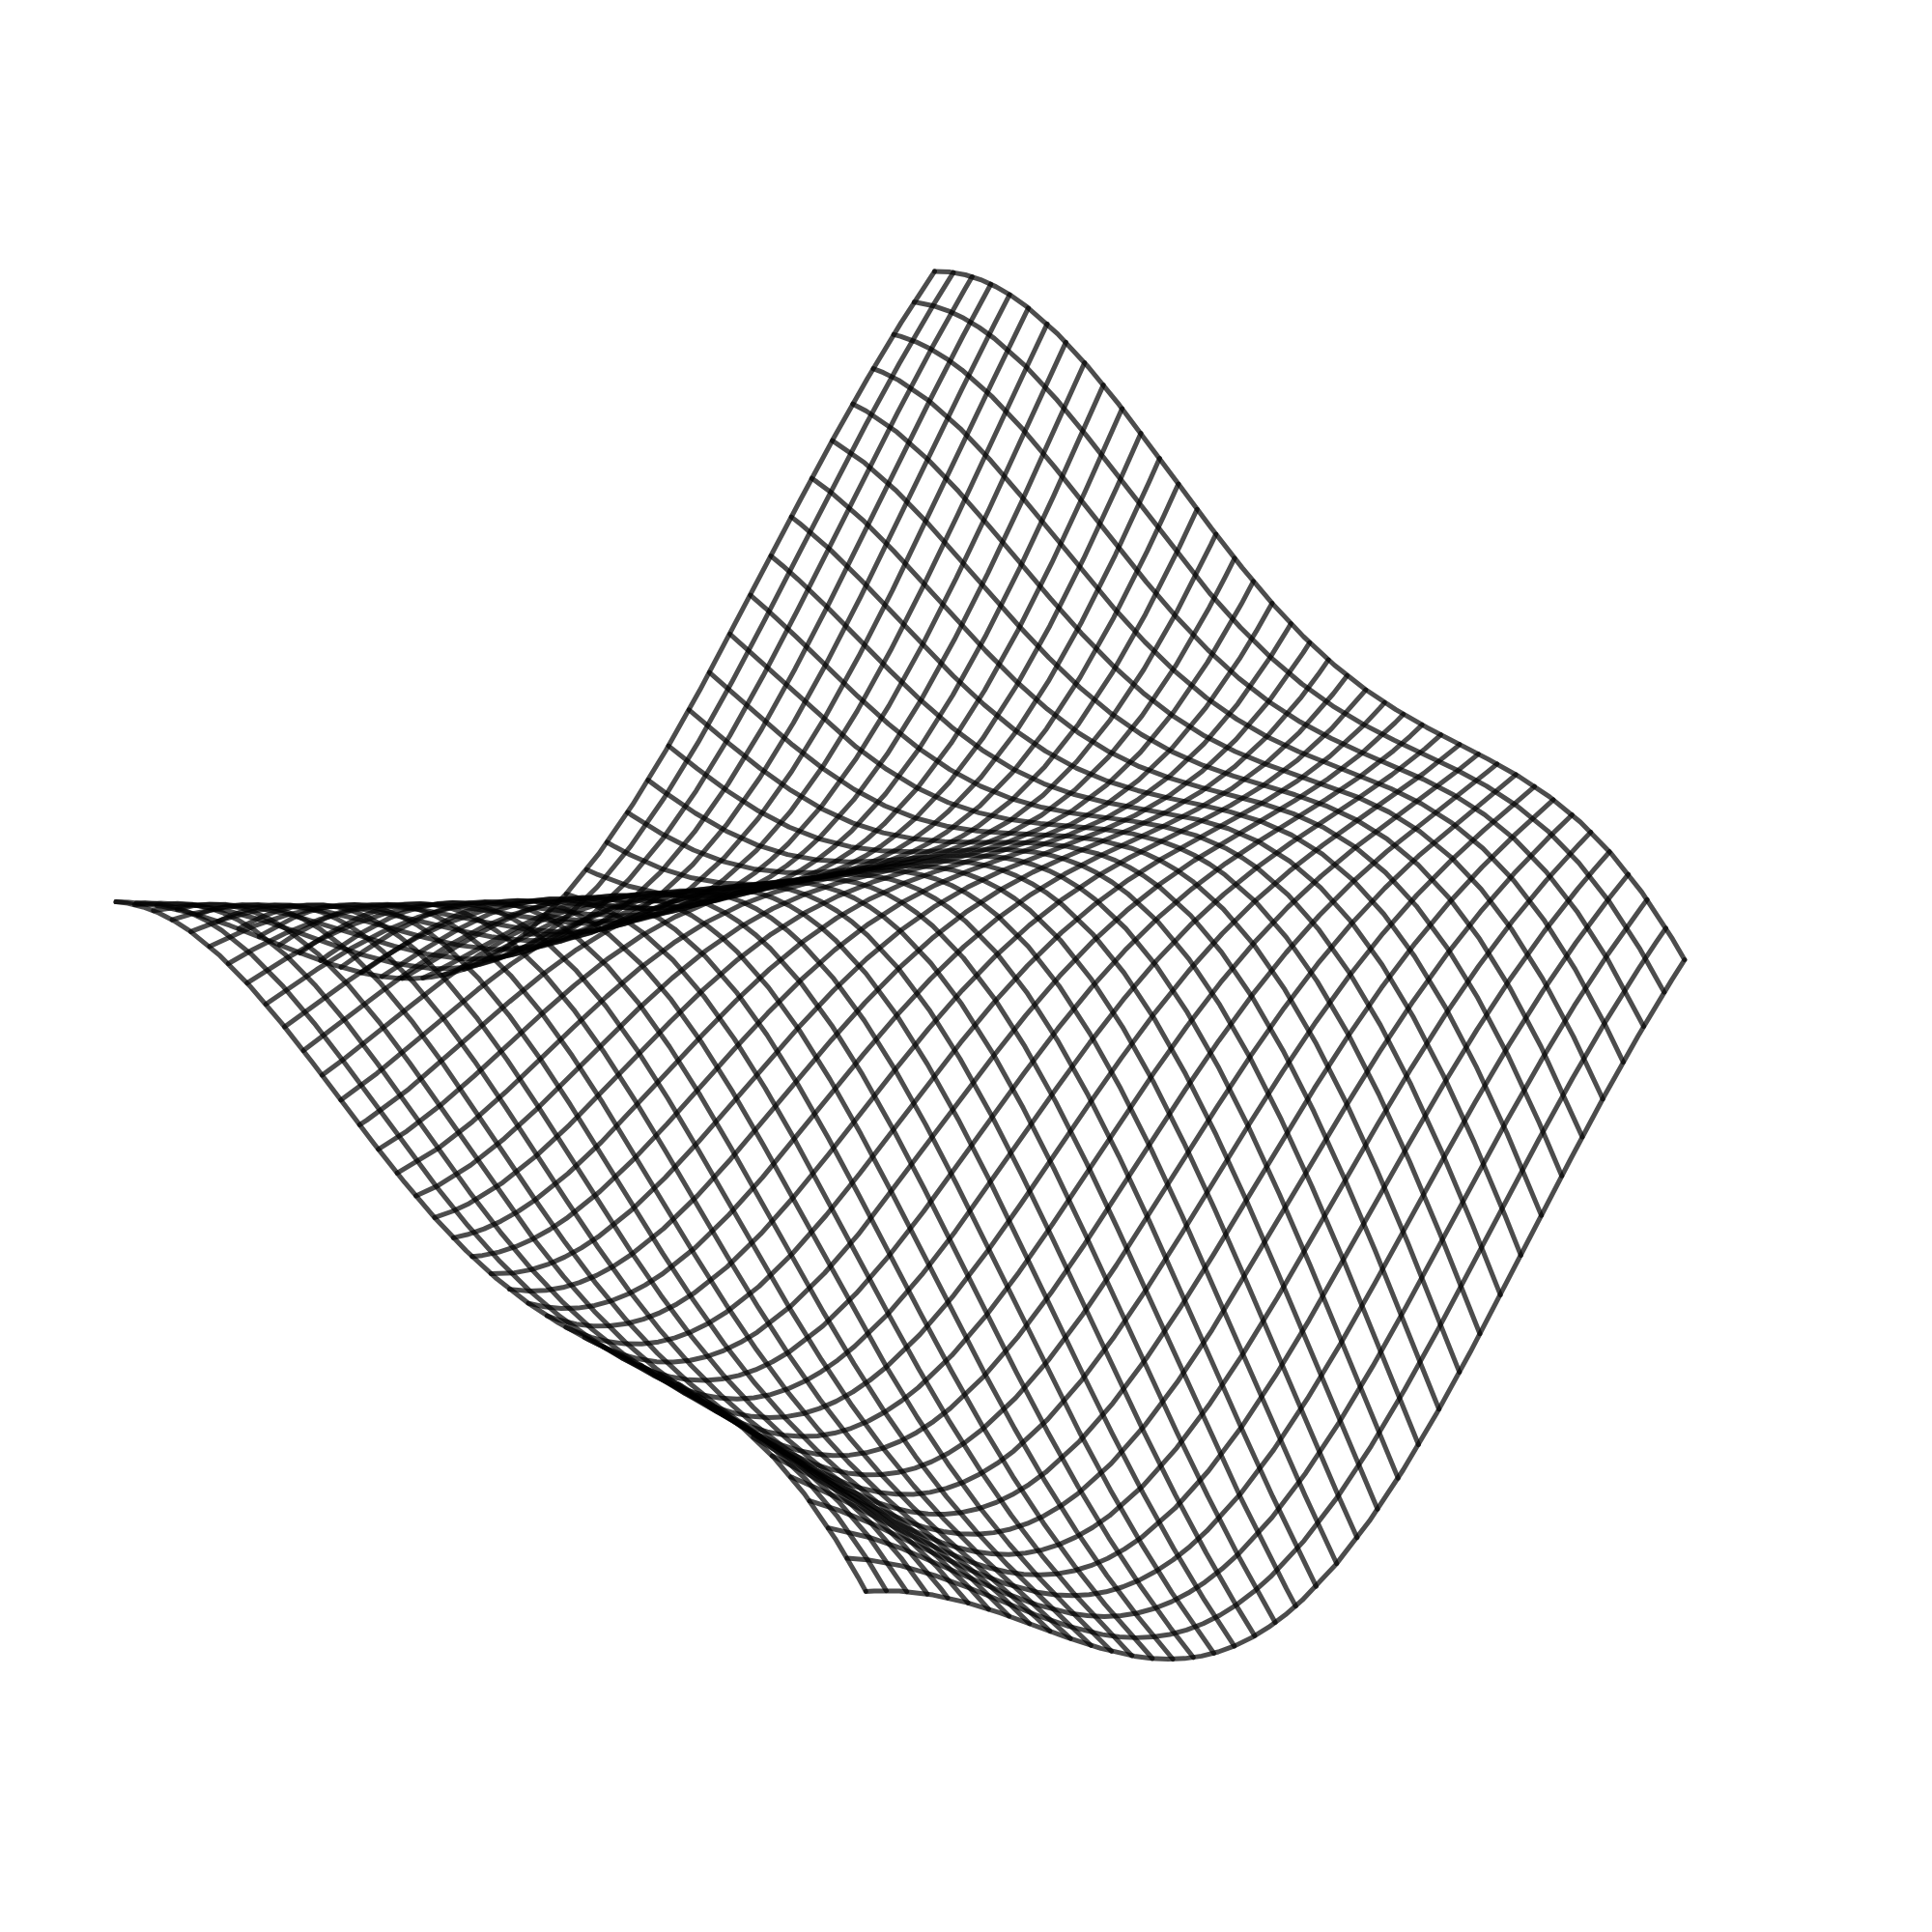
\includegraphics[width=0.9\linewidth]{img/m1/explicit.png}
  \caption{}
  \label{fig-explicit}
  \end{subfigure}
  \begin{subfigure}{0.5\linewidth}
    \centering
    
\includegraphics[width=0.8\linewidth]{img/m1/implicit.png}
    \caption{}
  \end{subfigure}
  \caption{(a) An explicit surface, given by $z = \cos ((x+y))+\frac{x^{2}}{6}-\frac{y^{2}}{6}$. (b) An implicit surface, given by $2 y\left(y^{2}-3 x^{2}\right)\left(1-z^{2}\right)+\left(x^{2}+y^{2}\right)^{2}-\left(9 z^{2}-1\right)\left(1-z^{2}\right)=0$. }
  \label{fig-imex}
\end{figure}

Apart from the explicit and implicit forms, surfaces can also be represented in their parametric form. The coordinates of a point $(x,y,z)$ of the surface patch are expressed as functions of parameters $u$ and $v$ in a closed rectangle:

\begin{equation}
x=x(u, v), \quad y=y(u, v), \quad z=z(u, v), \quad u_{1} \leq u \leq u_{2}, \quad v_{1} \leq v \leq v_{2}.
\end{equation}

In vector notation, the parametric surface can be specified by a vector-valued function

\begin{equation}
\mathbf{r}=\mathbf{r}(u, v)
\end{equation}

The parametric representation of surfaces is the most versatile out of the three. It is axis independent and is highly flexible in terms of defining complex intersections and point classification. It is generally easier to manipulate free-form shapes in parametric form than implicit or explicit forms  \cite{patrikalakis2009shape}. Hence, most of the CAD packages use parametric form of the surfaces to manipulate them. Bezier surface patch is one example of parametric form of a surface. 

\subsection{Surface File Format}


\begin{figure}
  \centering
  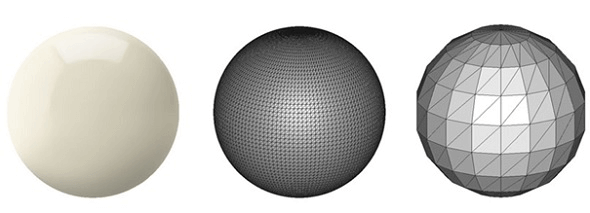
\includegraphics[width=\linewidth]{img/m1/tessellation.png}
  \caption{The perfect spherical surface on the left is approximated by tessellations. The figure on the right uses big triangles, resulting in a coarse model. The figure on the center uses smaller triangles and achieves a smoother approximation \cite{fileFormat}}
  \label{fig-tesellation}
\end{figure}

Given a free-form 3D surface geometry, various CAD packages could be used to encode it and store it in a file. Encoding the geometry using an approximate mesh is one of the most common methods adopted to store a surface geometry. An approximate mesh is created by covering the surface geometry with a series of tiny imaginary polygons. Trianlges are the most common polygon used for mesh generation. The encoded surface mesh can be stored in a file for sharing and future reference purposes. These files store the vertices of the triangles as well as the outward normal directions to the triangles. This process of tiling a surface with non-verlapping geometric shapes is also known as tessellation. Hence, the file formats used for storing the surface representation are called tessellated formats.

Due to the independent development of various CAD packages, a plethora of surface file formats are present in the mesh generation ecosystem. Many of these formats, such as DWG file format by AutoCAD and BLEND file format by Blender are proprietary. Hence, many of these cannot be shared between people working on different CAD packages. Native file formats are used to solve this problem. These formats can be shared easily among people working on different meshing softwares. One of the most common neutral surface file format is the STL (STereoLithography) file format. This format is compatible with most of the CAD and visualization softwares. Hence, we use the STL file format to import the surface geometry into our mesh generation algorithm.

An STL file stores the surface as a triangulated mesh. The following information is stored for all the triangles in teh STL file format:

\begin{enumerate}
  \item The coordinates of the vertices
  \item The components of the unit normal vector to the triangle pointing outwards with respect to the 3D model
\end{enumerate}

Surface triangulations

any commercial or open-source CAD package could be used to triangulate that surface. A fine triangular mesh can be considered as an approximate encoding of a given surface geometry. The approximation could be improved by increasing the number of triangles or decreasing their size. However, using smaller triangles results in larger number of triangles needed to tile the surface.


